% !TeX root = ../main.tex
% -*- coding: utf-8 -*-


\chapter{基于梯度上升决策树的函数抽取重构推荐} 
本章针对最常见的软件重构操作--函数抽取重构操作进行研究。本章首先阐述了函数抽取对完善软件系统设
计、提高软件质量的重要作用,然后介绍了本章的研究动机以及相关工作。针对研究动机中的问题描述,本章提出
了基于数据驱动的函数抽取重构推荐模型,模型中融合了内聚度、耦合度和复杂度的软件质量概念,并考虑了多种
程序元素。利用梯度上升决策树和逻辑斯特回归的融合模型,推荐函数抽取重构机会,从而帮助软件维护人员提高
维护效率。在实验部分,首先描述了实验设计,包括实验对象和评估方法。在对实验结果进行展示和分析后,讨论
了不同模型、数据集和特征对实验结果的影响,最后对本章进行小结。

\section{引言}
纠错性软件维护是保证软件正确性的重要手段,然而在纠错性维护后,虽然软件系统的正确性得以保障,但对软件
系统的修改可能会导致软件系统设计的偏离,使得软件质量降低。为了提高软件质量,通常需要后续进行完善性软
件维护。为了改进软件系统的设计,经常需要在不改变代码功能的前提下改变代码的结构,这种过程通常被称为软
件重构。软件重构作为一种重要的完善性软件维护手段,可以改善软件系统的设计、提高软件的易读性和可维护性
~\cite{fowler,mens:TSE04}。

大量的实践和研究表明,软件重构的作用主要有以下两种:(1)提高软件可维护性。当软件容易被理解时,软件
中的错误更容易被发现和修复~\cite{martin2009clean}。软件重构通过改进软件设计、重命名等方式,使得软件
设计更简单灵活、层次结构更清晰、代码更易被理解,从而减少代码维护的成本。(2)提高软件可扩展性。在软
件生命周期中,新的需求被不断添加,使得代码的复杂度越来越高,代码结构逐渐偏离原来的设计,从而导致了扩
展软件的难度越来越大。软件重构增加了程序设计的灵活性,通过改进软件设计,使得软件具备高内聚、低耦合和
复杂度低等特点,将复杂代码变简单,从而提高代码的可扩展性。

软件重构机会推荐作为一种自动化软件维护的手段,一直是研究者们较为关注的课题。软件重构机会推荐指的是推
荐软件系统中能够改善软件系统设计、提高软件质量但尚未被实施的重构机会
~\cite{fokaefs:icse11,higo:JSME,Liu:IEEE-TSE:12,Tourwe:CSMR03,Tsantalis:2011}。软件重构机会推荐可以
提高软件理解和维护的效率。Murphy-Hill等人~\cite{Murphy-Hill:ICSE09}对99个使用Eclipse集成开发工具的
Java开发人员进行了一个调研,发现函数抽取重构(Extract Method,简称EM)是最常用的软件重构类型之
一。函数抽取重构是在改变函数功能的前提下重新组织函数,把其中部分代码片段抽取出来并组成新的函数代替原
来的代码片段被调用。函数抽取重构的原因较为复杂,包括代码重用、长函数分解、重命名内部函数等11中主要原
因~\cite{silva2016we}。虽然函数抽取重构的原因较为复杂,但通常被抽取的代码段执行一个具体的、明确的功
能。正因为此,函数抽取重构通常可以改善软件系统的设计,提高易读性和可维护性。

虽然函数抽取重构被认为是最常被使用的软件重构类型之一~\cite{Murphy-Hill:ICSE09},但根据Kim等人的调研
报告,58.3\%的被调研者手动进行所有的函数抽取重构操作~\cite{Kim:FSE12}。同样,根据JDeodorant(著名的
重构机会推荐工具)的使用统计,函数抽取重构占所有被执行的重构操作的25\%,然而只有4.4\%的函数抽取重构
时通过Eclipse集成开发环境执行~\cite{Negara:ECOOP13,Murphy-Hill:ICSE09}。研究表明,开发和设计用于自动
推荐函数抽取重构机会的推荐系统可以在集成开发环境中发挥重要的作用~\cite{Tsantalis:2011}。

为了帮助软件维护人员提高软件重构的效率,研究者们开发了针对函数抽取重构的推荐工具。目前主流的函数抽取
重构机会推荐工具有:Fokaefs等人设计的JDeodorant~\cite{fokaefs:icse11},该工具基于程序切片技术选择可
以被提取到一个新函数的相关代码;Silva等人开发的JExtract~\cite{silva:CoRR15},根据最大化内聚度和最小
化耦合度的软件设计原则,设计了一个排序函数为候选函数抽取重构机会打分,抽取相对独立的、与剩余代码依赖
性较小的代码片段来组成新函数~\cite{silva:ICPC14};类似的,Charalampidou等人提出了
SEMI~\cite{charalampidou2016identifying},提取在距离在一定范围内的相关代码片段,并根据是否存在共同变
量来判断代码语句的相关性,最后针对所有的候选函数抽取重构机会,根据软件质量度量$LCOM_2$进行排序推荐。

尽管大多数函数抽取重构推荐技术旨在推荐改善软件设计的重构机会,但是由于软件设计的优劣和软件质量的好坏
很难通过具体的公式进行定义,以提高软件质量为目标的函数抽取重构推荐技术,大多通过特定的软件质量度量或
自定义函数对重构机会进行推荐,忽略了其它跟函数抽取重构相关的因素。然而函数抽取重构的原因较为复杂多
样,因此目前这些推荐方法的效果不甚理想。例如,软件质量度量LCOM(Lack of Cohesive Metric),只考虑了
具有共同变量的语句的个数作为内聚力的象征,而其它与函数抽取和程序功能相关的因素并没有被考虑进去。

本章提出基于机器学习的函数抽取重构机会推荐模型,通过提取一组结构特征和一组功能特征来对候选函数抽取重
构机会进行表示。具体来说,在特征提取算法中,提取了一组与函数和候选代码片段的复杂度相关的结构特征,以
及一组与内聚度和耦合度相关的功能特征。与传统的软件质量度量不同,该模型将软件质量相关的特征用一系列程
序元素来表示,包括与代码功能相关的变量使用、函数调用和包等。通过融合多种软件质量概念和程序元素,将函
数抽取重构机会表示为可供学习的特征序列。通过从开源软件仓库中挖掘真实存在的函数抽取重构实例,模型可以
从中学习到关于函数抽取重构的概率模型。给定一个新的函数体,该模型生成的候选函数抽取重构机会,并为每个
合法的重构机会分配一个概率,表示该重构机会为使用者所采纳的可能性,并按照概率由高至低进行推荐。

本章具有以下贡献:

(1)提出了一个关于函数抽取重构的概率模型,通过学习从开源软件仓库中挖掘到的重构实例,模拟了软件维护
人员进行软件重构的过程,并考虑了函数抽取重构原因的多样性。

(2)提出了关于结构特征和功能特征的特征提取算法,融合了内聚度、耦合度、复杂度的软件质量概念,并考虑
了多种程序元素。

(2)设计并开发了一个基于Eclipse的插件,为给定Java函数生成函数抽取重构机会,并为每个合法的候选重构机会
分配一个概率,按照概率由高至低推荐给集成开发环境使用者。

(3)在开源程序上与主流函数抽取重构推荐工具的对比实验证明了方法的有效性,能够更准确地推荐函数抽取重
构机会,为软件维护人员提高维护效率。

\section{相关工作与问题描述}
完善性软件维护是提高软件质量、保证软件可靠性和可维护性的重要手段。传统的软件质量度量方法从软件质量要
素出发,设计了一系列的度量标准来评估软件质量的好坏。目前主流的函数抽取重构机会推荐方法,通过软件质量
度量来评估候选重构机会的优劣,没有考虑其它与函数抽取重构相关的因素。本节首先对目前关于函数抽取重构机
会推荐的研究进行描述,然后通过示例阐述了基于软件质量度量的函数抽取重构机会推荐方法所存在的问题,最后
描述了本文的研究动机和思路。

\subsection{相关工作}
函数抽取重构推荐主要分为两个步骤:给定待重构的函数体,首先识别可以被抽取的代码段作为候选重构机会,然
后根据某种特定的方式将候选重构机会进行排序,并按序推荐给软件维护人员。因此,根据函数抽取重构的过程,
可以将关于函数抽取重构推荐的研究分为两个部分,分别是函数抽取重构机会识别和排序。本节从上述两个角度来总结和分析当前主流的函数抽取重构机会推荐方法。

\textbf{(1)函数抽取重构机会识别}

函数抽取重构机会识别指的是识别函数体中可以抽取的代码从而组成一个新的函数的代码,其本质是对函数体进行
拆分。目前关于识别函数抽取重构机会的研究主要分为基于程序语法和语义两种。

基于程序语法的函数抽取重构机会识别,主要通过程序切片的方式保证程序语法的正确性。Maruyama等人
~\cite{maruyama2001automated}首次提出使用程序切片来识别函数抽取重构机会,提出了个基于代码基本块的切
片方法对程序的控制流图进行切片。虽然该方法利用基本块来限制程序切片的范围,但由于其无法从语法上保证抽
取代码段前后程序的行为保持一致,因此其实用性受到了限制。为了保证函数抽取重构不会使程序行为发生改变,
Tsantalis和Chatzigeorgious~\cite{tsantalis2011identification}针对给定变量和对象,通过计算程序切片得
到所有可能改变变量的值或对象的状态的可执行切片。通过对程序切片的完全计算,该方法能够对给定的切片要求
(如某个特定的变量),在提取出所有与指定要求相关的代码片段的同时不改变原来的程序行为。

除了程序切片外,Yang等人~\cite{yang2009identifying}提出了针对规模较大的函数(``长函数''代码坏味)的
函数拆分方法,该方法根据函数的层次结构(如空行、分支和循环等)将长函数拆分成多个代码片段作为函数抽取
重构机会。Meananeatra~\cite{meananeatra2011using}等人定义了一组关于程序控制流和数据流的布尔表达式来
筛选被抽取的代码段,从而保证程序行为不变。例如,通过限制变量的定义和使用关系,确保变量在使用前已经被
定义,该方法可以过滤掉只包含某个变量的使用而不包含该变量定义的代码片段。Silva等人
~\cite{silva:ICPC14,silva:CoRR15}提出了基于代码块的函数抽取重构机会生成算法,将函数体表示为具有层次
结构的代码块的组合,每个代码块由顺序执行的子代码块组成。针对每个代码块,其中连续的子代码块组成一个候
选函数抽取重构机会。通过这样的方式,该算法能够生成所有能够顺序执行的代码片段,最终通过规则筛选出所有
合法的函数抽取重构机会。

基于程序语法的函数抽取重构机会识别,通常只能保证函数抽取重构后程序的语义和功能不发生改变,但仍然依赖
软件维护人员判断如何选取函数抽取重构机会(或指定切片条件)。根据``一个功能原则
''~\cite{martin2003agile}(Single Responsibility Principle,SRP),软件系统内的每个函数应该完成一个明确
的、特别的功能。基于这个原则,Charalampidou等人~\cite{charalampidou2016identifying}认为应该识别可能
完成某个特定功能的代码片段进行函数抽取重构。具体来说,他们认为在距离相近的有共同变量或函数调用的代码
语句在完成同一个功能,因此将这些语句视为一簇;通过合并重叠的小簇形成大簇,然后将每个大簇作为一个候选
重构机会。通过这种方法,他们认为能够识别所有可能在执行同一个程序功能的代码片段。然而,该方法在限制代
码之间距离的同时也限制了被抽取的代码片段的规模。例如,在代码片段中位置比较靠前的变量声明语句,由于距
离变量的使用存在一定距离,因此经常容易被忽略。除此以外,该方法在考虑代码功能的时候只考虑了变量和函数
调用,而没有考虑其它和代码功能相关的程序元素,如类型、包等。

\textbf{(2)函数抽取重构机会排序}

函数抽取重构是从给定函数体中抽取代码片段组成新函数并调用的过程。然而,能够抽取并保持程序行为不变的代
码片段通常有很多,尤其当函数规模变大时,其函数抽取重构机会的数量往往呈指数级上升。为了提高软件维护的
效率,部分研究对函数抽取重构机会进行排序,然后按序将候选重构机会推荐给使用者。

目前大部分关于函数抽取重构机会推荐的研究是根据函数级软件质量度量来对候选重构机会进行排序。软件质量度
量为从质量角度对软件系统的度量,其中与函数抽取重构相关的主要有复杂度、内聚度和耦合度等。根据SRP原
则,理想的函数抽取重构可以降低原函数的复杂度,使原函数和新函数具有较高的内聚度和较低的耦合度。

具体来说,基于复杂度的概念,部分研究使用函数复杂度(Method Complexity,MCX)来对函数抽取重构机会进行
排序~\cite{meananeatra2011using, yang2009identifying},倾向于推荐可以使函数复杂度尽可能小的重构机
会。基于内聚度的概念,部分研究使用函数内聚缺乏度(Lack of Cohesion of Method,LCOM)来评估函数抽取重
构对软件质量的改进程度,优先推荐让原函数和新函数的函数内聚缺乏度尽可能低的函数抽取重构机会
~\cite{meananeatra2011using, charalampidou2016identifying}。基于耦合度的概念,部分研究者提出优先推荐
尽可能独立的代码片段,使得重构之后原函数和新函数相关性尽可能小
~\cite{yang2009identifying,silva:ICPC14,silva:CoRR15},例如可以通过计算函数抽取时新函数所需要的参数
的数量来评估新函数对原函数的依赖性~\cite{yang2009identifying}。

与基于软件质量度量的方法不同,考虑到函数抽取重构原因的多样性~\cite{silva2016we}和软件质量度量的局限
性,本章提出构建关于函数抽取重构的概率模型,挖掘开源软件仓库中学习的重构实例,从中学习如何进行函数抽
取重构;除此以外,开发了``生成-排序''的推荐系统,为给定函数体生成所有合法的函数抽取重构机会,然后使
用训练好的模型为每个重构机会分配一个概率作为分数,按照分数由高至低进行推荐。与本章工作最相近的是
Silva等人的JExtract~\cite{silva:ICPC14,silva:CoRR15},该方法与本章方法的共同点是在识别函数抽取重构机
会的阶段不对重构机会进行筛选,而是依赖于后续的排序方法为使用者推荐重构机会;最大的区别是JExtract中的
排序算法假设被抽取的代码片段应该尽可能独立,因此JExtract计算待抽取代码与剩余代码之间的结构依赖性,推
荐尽可能独立的代码片段进行函数抽取重构。然而,软件维护人员进行函数抽取的原因多种多样
~\cite{silva2016we},只考虑结构依赖性作为函数抽取的原因在某些情况下存在一定的局限性。

\subsection{研究动机}
与纠错性软件件维护不同,完善性软件维护通常没有统一的、明确的标准来量化维护的效果。由于完善性软件维
护,尤其是软件重构的主要目的是改善软件系统的设计和提高软件质量,因此当前主流的面向函数抽取重构机会的
推荐技术采用软件质量度量作为评判重构机会的方法。然而,考虑到函数抽取重构的原因的多样性
~\cite{silva2016we}和软件质量度量的片面性,根据软件质量度量进行函数抽取重构机会推荐的效果往往不甚理
想。

\begin{figure}
\centering
\subfigure[函数抽取重构前函数]{\label{fig:before}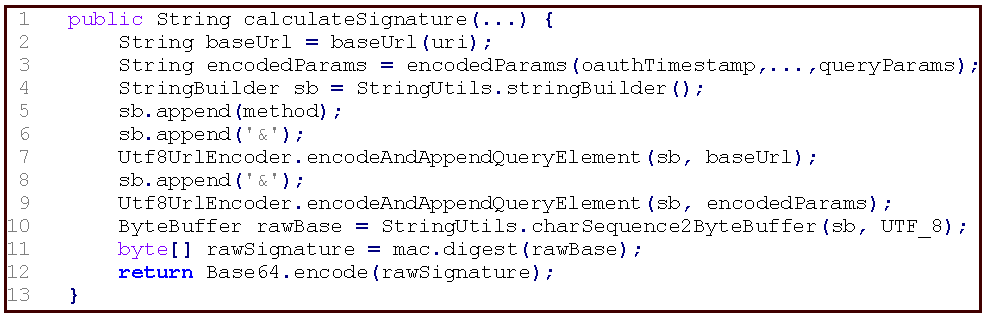
\includegraphics[width=0.98\linewidth]{before.pdf}}
\vskip\baselineskip
\subfigure[函数抽取重构后函数]{\label{fig:after}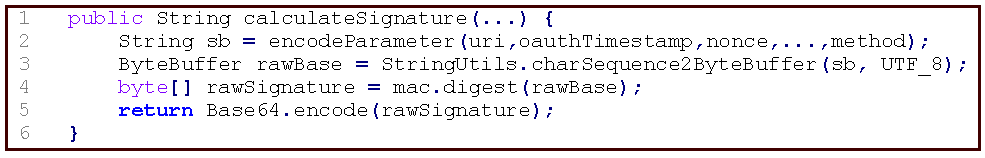
\includegraphics[width=0.98\linewidth]{after.pdf}}
\vskip\baselineskip
\subfigure[新函数]{\label{fig:new}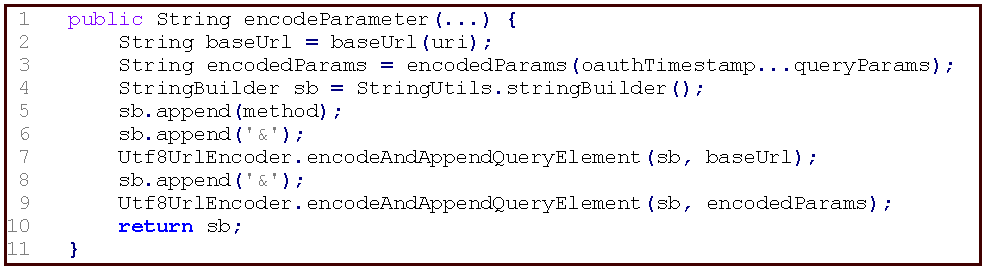
\includegraphics[width=0.98\linewidth]{new_cropped.pdf}}
\caption{函数抽取重构示例}
\label{refactor-example}
\end{figure}

图~\ref{refactor-example}为来自AsyncHttpClient库\footnote{AsyncHttpClient为处理Java应用HTTP请求的代
码库:\url{https://github.com/AsyncHttpClient/async-http-client}}的一个简单的重构示例。图
~\ref{fig:before}为重构前的函数$calculateSignature$,该函数的功能是计算HTTP签名。函数中第
2\textasciitilde9行实现了对参数进行编码的功能,并在接下来的版本中作为一个新的函数$encodeParameter$
(图~\ref{fig:new})被提取出来。图~\ref{fig:after}为函数抽取重构后的函数,可以看到在第2行通过调用新
函数,保持函数的语义和功能不发生改变。

\begin{table}[!t]
  \renewcommand{\arraystretch}{1.3}
  \caption{示例函数的函数抽取重构机会}
  \label{example_metrics}
  \centering
  \begin{tabular}{ccccc|ccccc}
  \toprule No.&Can&LCOM$_1$&LCOM$_2$&CPL &No.&Can&LCOM$_1$&LCOM$_2$&CPL\\ \midrule 1 &2-7 &8 &0 &6
   &9 &3-10 &6 &0 &6\\
   2 &2-8 &10 &0 &6 &10 &3-11 &13 &0 &6\\
   3 &\textbf{2-9} &11 &0 &6 &11 &3-12 &21 &0 &6\\
   4 &2-10 &13 &0 &6 &12 &4-9 &0 &0 &3\\
   5 &2-11 &28 &3 &6 &13 &4-10 &0 &0 &3\\
   6 &2-12 &36 &10 &6 &14 &5-7 &0 &0 &3\\
   7 &3-8 &4 &0 &6 &15 &5-8 &0 &0 &3\\
   8 &3-9 &5 &0 &6 &16 &5-9 &0 &0 &4\\
   \bottomrule
  \end{tabular}
\end{table}

为了模拟基于软件质量度量的函数抽取重构过程,表~\ref{example_metrics}中列出了函数$calculateSignature$
(如图~\ref{fig:before}所示)的16个候选函数抽取重构机会以及对应的软件质量度量。其中,Can为候选重构机
会,表~\ref{example_metrics}中使用起止代码行号来表示可被抽取的函数代码片段。表中列出了三种软件质量度
量方法,分别是函数内聚力缺乏度LCOM$_1$、LCOM$_2$和耦合度~\cite{yang2009identifying}。值得注意的是,
函数抽取重构中通常使用的LCOM$_1$和LCOM$_2$为描述函数体内部凝聚力的软件质量度量
~\cite{charalampidou2015size}。给定代码段$B$,$P$表示代码段中不共享任何变量的语句对的个数,$Q$为代码
段中存在共同变量的语句对的个数,则有$LCOM_1=P$。LCOM$_2$计算方式如下:
\begin{equation}\label{eq:lcom2}
      LCOM_2 = 
       \begin{cases}
             P-Q, & \textit{if}~P-Q\geq 0\\ 
  0, & elsewise,  
       \end{cases}
\end{equation}
不难看出,从函数体中抽取一个代码段,该代码段的LCOM$_1$和LCOM$_2$的值越低,表示其中不共享变量的语句对
越少,共享变量的语句对越多,此时代码段的内聚力越强。表~\ref{example_metrics}中的耦合度抽取该代码段时
所需要的参数的个数~\ref{yang2009identifying},因此耦合度越低,表示此时需要的参数越少,代码段与重构后
的原函数相关性较低,更符合软件设计原则。为由于示例代码的结构较为简单,因此表~\ref{example_metrics}中
未列出关于复杂度的软件质量度量。根据图~\ref{refactor-example}可知,在列出的16个函数抽取重构机会中只
有第3个重构机会(第2\textasciitilde9行)代表了最终抽取的代码片段。从表~\ref{example_metrics}中可以看
出,第12\textasciitilde16个代码段具有更低的函数内聚力缺乏度和耦合度,因此根据软件质量度量更适合被抽
取出来组成新函数;相反,相比较其它候选重构机会,第3个代码段在三个度量标准上均未有明显的优势,因此很
难通过软件质量度量来解释该代码段在后续版本中被抽取出来的原因。

因此,利用特定的软件质量度量来推荐函数抽取重构机会存在一定的局限性:(1)虽然软件质量度量是为了评价
软件质量而设计的,然而现有的度量标准往往只考虑某一种特定的程序元素,例如LCOM只考虑了使用共同变量的语
句的个数,而其它与软件质量相关的程序元素,如函数调用、类型和包等并没有被考虑进去。(2)函数抽取的目
的并不仅仅是为了提高软件质量度量或是减少代码坏味,还包括缺陷修复、方便新功能的添加或者提高程序易读性
等很难被量化的目的。因此通过某个软件质量度量或预定义的公式来进行函数抽取重构推荐,容易导致推荐的不准
确性。本章提出通过学习开源软件仓库中的重构实例,挖掘函数抽取重构的原因,构建关于函数抽取重构的概率模
型来推荐函数抽取重构机会。

\section{研究方法}
软件重构是完善性软件维护的重要手段。针对最常见的软件重构类型之一--函数抽取重构,本文提出了基于梯度上
升决策树的函数抽取重构机会推荐方法。本节首先介绍了方法的基本框架,然后提出了针对函数抽取重构实例的特
征提取算法,接着阐述了本文使用的梯度上升决策树和逻辑斯特回归融合模型,最后针对预测阶段给定函数体,阐
述了基于代码块的候选函数抽取重构机会生成的方法,并描述了模型预测和排序的过程。

\subsection{基本框架}
基于梯度上升决策树的函数抽取重构机会推荐,主要包括模型训练和重构推荐两个阶段。

\textbf{(1)训练阶段}

首先训练样本收集。为了挖掘函数抽取重构的原因,本章提出基于数据驱动的函数抽取重构机会推荐,通过对比开
源软件仓库中两个相邻的提交版本,收集函数抽取重构实例作为样本。然后针对训练样本集中的函数抽取重构实例
进行特征提取,根据特征提取算法将其表示为一个特征向量(feature vector)。最后训练模型。在将训练样本通
过特征提取算法表示完成后,利用基于梯度上升决策树和逻辑斯特回归的融合模型进行训练。

\textbf{(2)推荐阶段}

给定函数体,首先生成函数抽取重构机会,使用基于代码块的函数抽取重构机会生成算法,将所有在一个代码块内
的连续子块作为可能的函数抽取重构机会。然后筛选函数抽取重构机会。由于基于代码块的重构机会生成算法可能
生成破坏程序语义和功能的重构机会,因此使用基于规则的方法对函数抽取重构机会进行筛选,得到由所有合法重
构机会组成的集合。最后对函数抽取重构机会进行预测和排序推荐。针对集合中的每一个函数抽取重构机会,使用
训练好的模型预测其为训练样本中正例的概率,并根据概率由高至低进行排序,按序推荐给使用者。

值得注意的是,虽然本章方法需要一定的训练时间,但由于该训练过程是离线的,在训练完成后可以直接部署在集
成开发环境中,由使用者指定需要重构的函数,使用训练好的参数进行重构推荐,因此效率较高。

\subsection{特征提取算法}

给定训练样本集$\mathcal D$,其中第$i$个样本记为$D_i=(x_i,y_i)$,$x_i$表示``函数-代码片段''对,即$x_i=(m_i,f_i)$分别表示原函数$m_i$
和原函数中的一个代码片段$f_i$,记作$D_i=(m_i,f_i)$。

(2)针对函数抽取重构实例的结构和功能的改变,提取了两组特征--结构特征和功能特征,融合了包括复杂
度、内聚度和耦合度在内的软件质量因素,并考虑了多种程序元素。


\begin{figure}[bth]
  {
	\begin{center}
	  \begin{algorithmic} [1]
%                        \Procedure{feature\_extract}{$m,b,P$}
			\REQUIRE  : The input method \textit{m}, the selected block
			\textit{b} and the set of program elements \textit{P}
			\ENSURE The feature vector % \textit{feature\_extract(\textit{m},\textit{b},\textit{P})
			\STATE $S_M  \leftarrow getStmts(m)$
			\STATE $S_B  \leftarrow getStmts(b)$
			\FOR{$p$ in $P$}
				\STATE $E \leftarrow getElmts(b, p)$
				\FOR{$e$ in $E$}			
					\STATE $freq_M \leftarrow getFreq(m, e)$
					\STATE $freq_B \leftarrow getFreq(b, e)$
					\STATE $ratio_e \leftarrow freq_B / freq_M$
				\ENDFOR
				\STATE $idx \leftarrow \textit{idxOfMax}(ratio_E)$
				\STATE $cp \leftarrow ratio_{idx}$
				\STATE $loc \leftarrow getLOC(b)$				
				\STATE $count \leftarrow 0$				
				\FOR{$s$ in $S_B$}
					\IF{$E_{idx}$ in $getElmts(s)$}
						\STATE $count \leftarrow count + 1$
					\ENDIF
				\ENDFOR
				\STATE $ch \leftarrow count / loc$ 
				\STATE $setFeature(p, cp, ch)$
			        \ENDFOR
%                                \EndProcedure
		\end{algorithmic}
	\end{center}
        }
	\caption{特征提取算法}
	\label{feature_algorithm}
\end{figure}
\subsection{梯度上升决策树模型}
由于方法的最终目的是为给定函数生成候选重构序列,并按序推荐给使用者。然而,在挖掘开源软件
仓库时,能够得到的信息只有是否进行函数抽取重构,而没有相关的排序。因此,本文使用融合模型,利用最大似
然的方法估算候选函数抽取重构机会为正例的概率。

\subsection{候选函数抽取重构操作生成}
\subsection{预测}
\section{实验设计}
\subsection{实验对象}
\begin{table}[!t]
  \renewcommand{\arraystretch}{1.3}
  % if using array.sty, it might be a good idea to tweak the value of
  % \extrarowheight as needed to properly center the text within the cells
  \caption{Statistics of Subject Systems}
  \label{benchmark}
  \centering
  \begin{tabular}{ccc}
  \toprule 
  Projects &Methods &Refactor.\\ \midrule
  JHotDraw &56 &56 \\ 
  Junit &25 &25 \\ 
  MyWebMarket &23 &35 \\ 
  SelfPlanner &12 &13 \\ 
  Wikidev &14 &26 \\ \midrule
  Total &130 &155 \\ 
  \bottomrule
  \end{tabular}
  \end{table}

\subsection{实验方法}
通过对没有被重构的函数随机抽取代码片段,得到负样本集。

为在原函数中存在的、在后一个版本中被抽取出来作为新函数的代码片段

给定两个相邻的版本,$P$表示其中较早的一个版本,$P'$表示另一个版本。假定版本$P$中存在一个函数$M$,函
数中的一个代码片段$F$在版本$P'$中被抽取出来组成一个新的函数被原函数$M$调用,则函数$M$和代码片段$F$组
成一个重构实例。
\subsection{评估指标}

\section{实验结果与分析}

\begin{table}[!t]
  \renewcommand{\arraystretch}{1.3}
  % if using array.sty, it might be a good idea to tweak the value of
  % \extrarowheight as needed to properly center the text within the cells
  \caption{Accuracy of Different Approaches}
  \label{accuracy}
  \centering
  \begin{tabular}{cc|ccc}
  \toprule
   Tools &Tolerance &Precision &Recall &F-measure\\ 
  \hline
  \multirow{4}{*}{GEMS$^{GB}$}&$1\%$ &\bf{22.5\%} &\bf{54.2\%} &\bf{31.8\%} \\ 
  &$2\%$ &\bf{28.5\%} &\bf{59.8\%} &\bf{38.6\%} \\ 
  &$3\%$ &\bf{34.3\%} &\bf{62.6\%} &\bf{44.3\%} \\ 
  \hline
  \multirow{4}{*}{JExtract}&$1\%$ &12.6\% &52.2\% &20.4\% \\ 
  &$2\%$ &13.1\% &\bf{59.3\%} &21.5\% \\ 
  &$3\%$ &15.0\% &61.9\% &24.2\% \\ 
  \hline
  \multirow{4}{*}{SEMI}&$1\%$ &12.9\% &38.0\% &19.2\% \\ 
  &$2\%$ &14.6\% &47.0\% &22.3\% \\ 
  &$3\%$ &18.8\% &55.5\% &28.1\% \\ 
  \hline
  \multirow{4}{*}{JDeodorant}&$1\%$ &17.4\% &14.8\% &16.0\% \\
  &$2\%$ &21.1\% &18.4\% &19.7\% \\ 
  &$3\%$ &28.0\% &23.8\% &25.7\% \\ 
  \bottomrule
  \end{tabular}
  \end{table}

\begin{table}[!t]
  \renewcommand{\arraystretch}{1.3}
  % if using array.sty, it might be a good idea to tweak the value of
  % \extrarowheight as needed to properly center the text within the cells
  \caption{Accuracy in Long methods}
  \label{long_methods}
  \centering
  \begin{tabular}{cc|ccc}
  \toprule
   Tools &Tolerance &Precision &Recall &F-measure\\ 
  \hline
  \multirow{4}{*}{GEMS$^{GB}$}&$1\%$ &13.3\% &31.9\% &18.8\% \\ 
  &$2\%$ &\bf{17.4\%} &\bf{41.5\%} &\bf{24.5\%} \\ 
  &$3\%$ &\bf{25.3\%} &\bf{46.2\%} &\bf{32.7\%} \\ 
  \hline
  \multirow{4}{*}{JExtract}&$1\%$ &6.6\% &16.1\% &9.4\% \\ 
  &$2\%$ &8.0\% &19.3\% &11.3\% \\ 
  &$3\%$ &8.0\% &19.3\% &11.3\% \\ 
  \hline
  \multirow{4}{*}{SEMI}&$1\%$ &\bf{16.4\%} &\bf{38.7\%} &\bf{23.0\%} \\ 
  &$2\%$ &\bf{17.9\%} &\bf{41.9\%} &\bf{25.0\%} \\ 
  &$3\%$ &19.1\% &45.1\% &26.9\% \\ 
  \hline
  \multirow{4}{*}{JDeodorant}&$1\%$ &12.0\% &9.6\% &10.7\% \\
  &$2\%$ &14.3\% &12.9\% &13.5\% \\ 
  &$3\%$ &16.0\% &12.9\% &14.2\% \\ 
  \bottomrule
  \end{tabular}
  \end{table}

\section{讨论}
\section{系统展示}
\section{本章小结}
虽然已经开发完成的Eclipse插件是面向Java语言的,但只需要改变特征向量的生成方式,,本章方法可同样适用
于其它语言。Hence, our approach learns a model to capture the common characteristics of Extract
Method refactorings. We also propose two important functionality-related features to learn the
model: (1) {\em Coupling-related features}: this assesses the extent to which the extracted code is
performing a unique functionality than the remaining code; and (2) {\em Cohesion-related features:}
It assesses the extent to which the extracted code is involved in providing a specific
functionality.

提出了关于函数抽取重构的特征提取算法,该算法为每个训练样本提取两组特征,分别是结构特征和
功能特征,融合了软件质量的概念和多种与函数抽取重构相关的程序元素;接着阐述了使用的梯度上升决策树和逻
辑斯特回归融合模型。在预测阶段,阐述了根据给定函数体生成候选函数抽取重构机会的方法以及最后的概率预测
和排序方法。